\documentclass[a4paper, 12pt]{report}

\usepackage{german}
\usepackage{bookman}
\usepackage[T1]{fontenc}
\usepackage[utf8]{inputenc}
\usepackage{./custompkg}
\usepackage{xcolor}
\usepackage{graphicx}

\begin{document}
	\thispagestyle{empty}
	
	\bslinespacing{1.5}
	{
		\centering
		\Huge
		\color{blue}
		Anleitung
	}
	
	\centering
	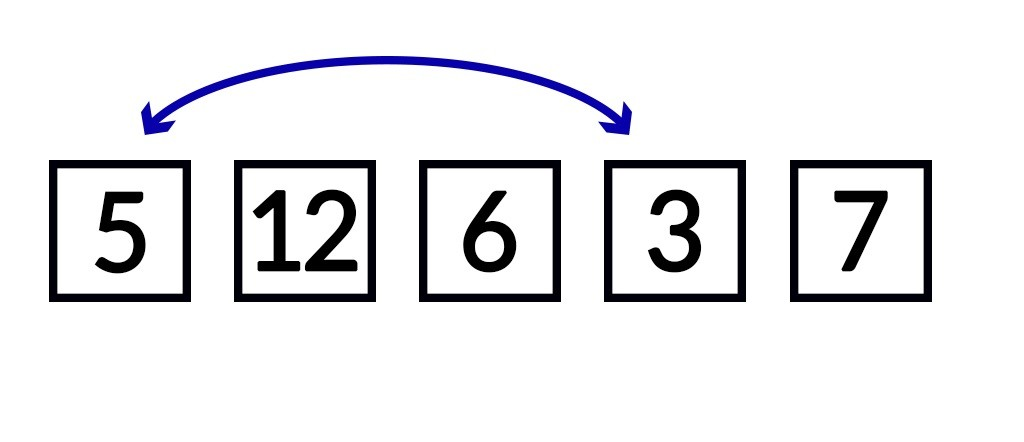
\includegraphics[width=5cm]{IMG_1125.JPG}
	\raggedright
	\paragraph{\color{blue}Materialien} \mbox{} \\
	\begin{itemize}
		\item mind. 2 Blätter A4-Papier mit unterschiedlichen Nummern bedruckt.
	\end{itemize}
	
	\raggedright
	\paragraph{\color{blue}Anleitung} \mbox{} \\
	\begin{enumerate}
		\item Jeder Schüler erhält ein Blatt
		\item Die Schüler stellen sich in einer unsortierten Reihenfolge auf.
		\item Es wird sich für einen Sortieralgorithmus entschieden.
		\item Die Schritte des gewählten Algorithmuses werden nacheinander durchgeführt, bis die Schüler in der sortierten Reihenfolge stehen.
	\end{enumerate}
	
	\raggedright
	\paragraph{\color{blue}Erklärung} \mbox{} \\
	
	Ein Algorithmus ist eine Reihenfolge von Anweisungen, die zu einem gewissen Ziel führen.
	Dieser kann dazu verwendet werden ein gewisses Problem zu lösen.
	Ein Sortieralgorithmus ist, wie der Name schon sagt, dafür da, eine Datenmenge in die richtige Reihenfolge zu bringen.
	Es gibt verschiedene Sortieralgorithmen, die unterschiedlich schnell bzw. effizient sind. Ein sehr einfacher Algorithmus ist der Bubble-Sort-Algorithmus. 	
\end{document}